\chapter{Theory}

\section{Introduction}

In this chapter a brief historical background of the Standard Model is given
with some of the results that inform our current understanding. The role of
symmetry in particle physics is discussed and the gauge structure of the
Standard Model is examined. The motivation for new physics at the TeV scale is
considered. A brief description of supersymmetry, a popular possible extension 
to the Standard Model, is given and the ideas behind it are discussed. Finally,
the current exclusion limits on Gauge Mediated SUSY Breaking are reviewed. 

\section{The Standard Model}

The Standard Model of particle physics contains our theoretical knowledge of the
fundamental particles and the forces between them. Figure \ref{fig:particles}
shows the fundamental particles and the force carriers according to our current
knowledge. \\

\begin{figure}
\begin{center}
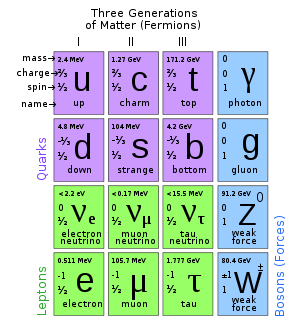
\includegraphics[width=0.6\textwidth]{particles.png}
\end{center}
\caption{The fundametal particles according to the Standard Model.}
\label{fig:particles}
\end{figure}

Historically the Standard Model was formed by trying to understand atomic
spectra. In 1928 Dirac came up with the Dirac equation to describe fermions, 
which was the first theory to deal with relativity and quantum mechanics. Later 
QED a theory of the interactions of light with matter was developed by Richard 
Feynman (among others) which explained the Lamb shift in Hydrogen and made a 
very precise prediction for the magnetic moment of the electron. \\

The neutrino was postulated by Pauli in 1930 to explain the continuous electron 
energy spectrum in $\beta$-decay. Neutrinos were discovered by direct detection 
in 1956 by beta capture in a huge detector of water with CdCl$_{2}$ dissolved in
it by the Savannah River nuclear reactor. Three flavours of neutrinos 
corresponding to each of the leptons has been discovered. More recently neutrino 
oscillations have been observed in which neutrinos can change flavour. The 
flavour change happens due to a diffenece between the mass eigenstates and the 
flavour eigenstates indicating that neutrinos have a non-zero mass. \\

After the discovery of many new hadrons, e.g. $\pi$, K, $\Delta$, $\Sigma$, it
became clear that the neutron and proton are not fundamental particles, but made
up of more basic constituents. Gell-Mann came up with the quark model in which 
all hadrons are made up of quarks. There are 6 flavours of quarks with different
masses: u, d, c, s, t, b. Each flavour of quark comes in three different colors.
Quarks carry color charge and form an SU(3) color triplet. Quarks are not 
observed as free particles, but only in colorless bound states. \\

A beautiful experiment by C. S. Wu and collaborators showed that parity is
violated in weak interactions. The beta decay of $\mbox{Co}^{60}$ was performed 
in a magnetic field and at low temperature to polarise the nuclei and the 
angular distribution of electrons was measured. An asymmetry in the distribution
between $\theta$ and $180^{\circ} - \theta$ (where $\theta$ is the angle between 
the electron momentum and the orientation of the parent nucleus) was observed
providing unequivocal proof that parity is not conserved in beta decay. This is
represented in the Standard Model by the presence of chiral fermions in the
structure of the weak interaction. \\

Electroweak theory was introduced by Glashow, Salam and Weinberg who proposed
that the electromagnetic force and the weak force are parts of the same theory. 
The $W^{\pm}$ and $Z^{0}$ bosons were predicted to have have masses in the ratio
$\frac{m_{W}}{m_{Z}} = \cos{\theta_{W}}$, where $\theta_{W}$ is the weak mixing 
angle. The $W^{\pm}$ and $Z^{0}$ bosons were discovered by the UA1 and 
UA2 experiments at CERN. Carlo Rubbia and Simon van der Meer won the Nobel Prize
for Physics in 1983 for their decisive contributions toward the discovery. \\

The Large Electron Positron Collider (LEP) made $e^{+}e^{-}$ collisions to
search for new physics and make precision electroweak measurements. The
collision centre of mass energy could be tuned to generate a resonance of Z
bosons. Looking at the Z width for deacys to invisible particles relative to the
total Z width indicates that there are exactly three flavours of neutrino into
which the Z can decay. 

\section{Gauge Symmetries of the Standard Model}

There is an important connection between symmetries and conservation laws
discovered by Noether \cite{noether}.

\begin{center}
{\it For every symmetry of the theory there is a conserved quantity.} \\
\end{center}

Invariance under translations in time and space give rise to energy and momentum
conservation. Invariance uder rotation gives rise to conservation of angular
momentum. Together with Lorentz invariance these transformations form the
Poincare group. Describing symmetries in terms of group theory was developed by
Galois in the 19th Century and was initially used to test the solvability of 
polynomial equations \cite{galois}. These symmetries are all global symmetries
meaning that the transformation is the same for all space-time points. \\

A theory can be described by a Lagrangian which is equal to the kinetic energy
minus the potential energy. The equations of motion of such a theory can be
derived by minimising the action (Equation \ref{eq:action}).

\begin{equation}
S = \int L d^{4}x^{\mu}
\label{eq:action}
\end{equation}

Consider a Lagrangian with N scalar fields $\mathbf{\phi}(x^{\mu}) =
\left(\phi_{1}(x^{\mu}),...,\phi_{N}(x^{\mu})\right)$, where $x^{\mu}$ is the
space-time co-ordinate as in Equation \ref{eq:lagrangian}.

\begin{equation}
L = L(\mathbf{\phi}, \partial_{\mu}\mathbf{\phi}, x^{\mu})
\label{eq:lagrangian}
\end{equation}

Suppose that this Lagrangian is invariant under the gauge transformation given
in Equation \ref{eq:gauge}, where the phase is composed of the parameters 
$\epsilon^{a}\left(x^{\mu}\right)$ and the generators of the Lie group $T^{a}$. 
This is a gauge symmetry rather than a global symmetry since the phase depends 
on the space-time point. 

\begin{equation} 
\phi(x^{\mu})\rightarrow \phi(x^{\mu})e^{-i\epsilon^{a}T^{a}}
\label{eq:gauge}
\end{equation}

Noether's theorem gives a powerful way of constructing theories based on 
symmetry which underpins the structure of the standard model. The gauge
symmetry of the Standard Model is $SU(3)\times SU(2)\times U(1)$. SU(3) 
corresponds to QCD and $SU(2)\times U(1)$ corresponds to the electroweak
sector. Much of the structure of the Standard Model can be understood by 
considering the gauge groups.

\subsection{Quantum Electrodynamics (QED)}

The QED Lagrangian for electromagnetic interactions of electrons can be written 
as Equation \ref{eq:qed}.

\begin{equation}
L = -\frac{1}{4}F_{\mu\nu}F^{\mu\nu} + \bar{\psi}\gamma^{\mu}D_{\mu}\psi
- m_{e}\bar{\psi}\psi
\label{eq:qed}
\end{equation} 

The first term represents the free electromagnetic field. $F_{\mu\nu} = 
\partial_{\mu}A_{\nu} - \partial_{\nu}A_{\mu}$, where $A_{\mu}$ is the 
electromagnetic vector potential. The second term reresents the electron kinetic 
energy and the interaction between electron and photon. $D_{\mu} = 
\partial_{\mu} - ieA_{\mu}$ is the covariant derivative (i.e. it remains the 
same under the gauge transformation). The third term represents the mass of the 
electron. This lagrangian is invariant under the U(1) gauge transformation given 
by Equation \ref{eq:transformations}.

\begin{eqnarray}
\psi &\rightarrow& e^{-i\alpha(x)}\psi \\
A_{\mu}   &\rightarrow& A_{\mu} + \frac{1}{e}\partial_{\mu}\alpha(x)
\label{eq:transformations}
\end{eqnarray}

The mass term for the electron is allowed by gauge invariance, but a mass term for 
the photon is forbidden. Also photon self-interactions are forbidden by gauge 
invariance. The constraints set by gauge invariance tell us a lot about the
nature of the electromagentic interaction. The photon is a massless particle which 
interacts with electrons, but not with itself. The electromagnetic force has 
infinite range. \\

QED has been tested to very high precision. Consider the magnetic moment of the
electron given by Equation \ref{eq:emagmom}.

\begin{equation}
\vec{\mu} = -\frac{g\mu_{B}\vec{S}}{\hbar}
\label{eq:emagmom}
\end{equation}

where $\mu_B$ is the Bohr magneton, $\hbar$ is the Planck constant, $\vec{S}$ is
the electron spin and $g$ is a constant factor. \\

According to Dirac's theory $g = 2$, however QED predicts quantum corrections to
this value. The QED prediction agrees with the experimentally measured value 
\cite{qed} to more than 10 significant figures:

\begin{equation}
\frac{g - 2}{2} = 0.00115965218073(28)
\end{equation}


\subsection{The Electroweak Sector}

The electroweak force consists of SU(2) weak isospin and U(1) hypercharge. Table 
\ref{tab:ewk} defines the symbols for the groups, the corresponding fields and 
the generators. \\

\begin{table}
\begin{center}
\begin{tabular}{|c|c|c|c|}
\hline
Group & Fields & Strength & Generators \\
\hline
SU(2) & $A_{\mu}^{a}$ & $g$ & $T^{a} = \frac{\sigma^{a}}{2}$ \\
U(1) & $B_{\mu}$ & $g^{\prime}$ & $Y = \frac{1}{2}$ \\
\hline
\end{tabular}
\end{center}
\caption{Definitions of the symbols represting the properties of the electroweak
groups. $a = 1, 2, 3$ and $\sigma^{a}$ are the Pauli matrices.}
\label{tab:ewk}
\end{table}

Consider a scalar field doublet, $\phi$, with respect to SU(2) with U(1) 
hypercharge $Y = \frac{1}{2}$. The bosonic sector of the electroweak lagrangain 
can be written as:

\begin{equation}
L = -\frac{1}{4}F_{\mu\nu}^{a}F_{\mu\nu}^{a}
-\frac{1}{4}G_{\mu\nu}G_{\mu\nu} + (D_{\mu}\phi)^{\dagger}(D_{\mu}\phi) -
\lambda\left(\phi^{\dagger}\phi - \frac{v^{2}}{2}\right)
\label{eq:ew}
\end{equation}

where
\begin{eqnarray}
F_{\mu\nu}^{a} &=& \partial_{\mu}A_{\nu}^{a} - \partial_{\nu}A_{\mu}^{a} +
g\epsilon^{abc}A_{\mu}^{b}A_{\nu}^{c} \\
G_{\mu\nu} &=& \partial_{\mu}B_{\nu} - \partial_{\nu}B_{\mu} \\
D_{\mu}\phi &=& \partial_{\mu}\phi - i\frac{g}{2}\sigma^{a}A_{\mu}^{a}\phi -
i\frac{g^{\prime}}{2}B_{\mu}\phi
\end{eqnarray}

There is a continuum of ground states giving equivalent physics, one of which
must be chosen by nature. This is known as symmetry breaking. Arbitrarily 
choose:

\begin{equation}
A_{\mu} = 0 \hspace{2cm} B_{\mu} = 0 \hspace{2cm} \phi_{0} =
\frac{v}{\sqrt{2}}\left(\begin{array}{c}0\\1\end{array}\right)
\end{equation}

Finding the unbroken generator, Q, such that $Q\phi_{0} = 0$ and Q is hermitian
gives:

\begin{equation}
Q = \left(\begin{array}{cc}1&0\\0&0\end{array}\right)
\end{equation}
or
\begin{equation}
Q = T^{3} + Y 
\end{equation}

The unbroken generator corresponds to the subgroup U(1)$_{em}$ of
SU(2)$\times$U(1). This should correspond to a massless gauge field -- the
electromagnetic field. U(1)$_{em}$ is not the same as the U(1) component in
SU(2)$\times$U(1) so the electromagnetic potential, $A_{\mu}$ (without
superscript) is not $B_{\mu}$, but a linear combination of the fields
$A_{\mu}^{3}$ and $B_{\mu}$. \\

Consider small perturbations around the ground state:

\begin{equation}
\phi = \left(
\begin{array}{c}
0 \\ 
\frac{v}{\sqrt{2}} + \frac{\chi(x)}{\sqrt{2}}
\end{array}
\right)
\end{equation}

Thus we get the following expression for $D_{\mu}\phi$:

\begin{equation}
D_{\mu}\phi = \left(
\begin{array}{c}
-\frac{ig}{2\sqrt{2}}\left(A_{\mu}^{1} - iA_{\mu}^{2}\right)(v + \chi(x)) \\
-\frac{i}{2\sqrt{2}}\left(g^{\prime}B_{\mu} - gA_{\mu}^{3}\right)(v + \chi(x)) +
\frac{1}{\sqrt{2}}\partial_{\mu}\chi(x)
\end{array}
\right)
\end{equation}

Introduce new fields:
\begin{eqnarray}
W_{\mu}^{\pm} &=& \frac{1}{\sqrt{2}}(A_{\mu}^{1} \mp A_{\mu}^{2}) \\
Z_{\mu} &=& \frac{1}{\sqrt{g^{2} + g^{\prime 2}}}(gA_{\mu}^{3} -
g^{\prime}B_{\mu}) = \cos\theta_{W}A_{\mu}^{3} - \sin\theta_{W}B_{\mu} \\
A_{\mu} &=& \frac{1}{\sqrt{g^{2} + g^{\prime 2}}}(gB_{\mu} -
g^{\prime}A_{\mu}^{3}) = \sin\theta_{W}A_{\mu}^{3} + \cos\theta_{W}B_{\mu}
\end{eqnarray}

$Z_{\mu}$ and $A_{\mu}$ are rotations of the original fields with angle
$\theta_{W}$ which satisfies Equation \ref{eq:thetaw}.

\begin{equation}
\cos\theta_{W} = \frac{g}{\sqrt{g^{2} + g^{\prime 2}}} \hspace{2cm}
\sin\theta_{W} = \frac{g^{\prime}}{\sqrt{g^{2} + g^{\prime 2}}}
\label{eq:thetaw}
\end{equation}

$Z_{\mu}$ and $A_{\mu}$ are determined by the necessity that the covariant
derivative, $D_{\mu}\phi$, does not contain $A_{\mu}$ -- it must be invariant
under the electromagnetic gauge transformation. To quadratic order the
lagrangian can be written as:  

\begin{eqnarray}
L = -\frac{1}{2}\mathcal{W}_{\mu\nu}^{+}\mathcal{W}_{\mu\nu}^{-} + 
m_{W}^{2}W_{\mu}^{+}W_{\mu}^{-} \\
-\frac{1}{4}\mathcal{Z}_{\mu\nu}\mathcal{Z}_{\mu\nu} + 
\frac{m_{Z}^{2}}{2}Z_{\mu}Z_{\mu} \\
-\frac{1}{4}F_{\mu\nu}F_{\mu\nu} \\
+\frac{1}{2}(\partial_{\mu}\chi)^{2} - \frac{m_{\chi}^{2}}{2}\chi^{2}
\end{eqnarray}

where
\begin{eqnarray}
\mathcal{W}_{\mu\nu}^{\pm} &=& \partial_{\mu}W_{\nu}^{\pm} -
\partial_{\nu}W_{\mu}^{\pm} \\
\mathcal{Z}_{\mu\nu} &=& \partial_{\mu}Z_{\nu} - \partial_{\nu}Z_{\mu}
\end{eqnarray}

The physical fields can be seen from the lagrangian and are summarised in Table
\ref{tab:physical}. \\

\begin{table}
\begin{center}
\begin{tabular}{|c|c|c|}
\hline
Field & Mass & Particle \\
\hline
$W_{\mu}^{\pm}$ & $m_{W} = \frac{gv}{2}$ & $W^{\pm}$ \\
$Z_{\mu}$ & $m_{Z} = \frac{\sqrt{g^{2} + g^{\prime 2}}v}{2}$ & $Z^{0}$ \\
$A_{\mu}$ & $m_{\gamma} = 0$ & $\gamma$ \\
$\chi$ & $m_{\chi} = \sqrt{2\lambda}v$ & Higgs \\
\hline
\end{tabular}
\end{center}
\caption{The physical fields from electroweak symmetry breaking.}
\label{tab:physical}
\end{table} 

The electroweak theory of Glashow, Salam and Weinberg predicted mixing between
the electromagnetic and weak forces and the existence of $W^{\pm}$ and $Z^{0}$ 
bosons with masses in the ratio given by Equation \ref{eq:masses}. 

\begin{equation}
\frac{m_{W}}{m_{Z}} = \cos\theta_{W}
\label{eq:masses}
\end{equation}

The electric charge is connected to the weak mixing angle by:

\begin{equation}
e = g\sin\theta_{W}
\end{equation}

The existence of the $W^{\pm}$ and $Z^{0}$ bosons was confirmed experimentally 
by the UA1 and UA2 experiments in CERN. The masses were measured to be:

\begin{equation}
m_{W} = 80.4\pm \GeV \hspace{2cm} m_{Z} = 91.2\pm \GeV
\end{equation}

The weak mixing angle, $\theta_{W}$, was measured independently to satisfy 
$\sin\theta_{W} = 0.23$ in good agreement with the predictions of the
electroweak theory. \\

Both leptons and quarks feel the weak interaction. The $W^{\pm}$ interact only
with left-handed fermions. Handedness (or chirality) is the eigenvalue of the 
$\gamma^{5}$ matrix. It corresponds to the helicity (the projection of the spin 
onto the direction of motion) in the relativistic limit $m << E$. The left
handed and right handed components of a fermion $\psi$ can be projected out
using the operators $\frac{1}{2}(1 - \gamma^{5})$ and $\frac{1}{2}(1 + 
\gamma^{5})$ respectively. \\

The left handed components form SU(2) doublets while the right handed components
are singlets under SU(2) as in Equation \ref{eq:leptons} for leptons and
Equation \ref{eq:quarks} for quarks.

\begin{equation}
E_{L} = \left(\begin{array}{c}e\\\nu_{e}\end{array}\right)_{L} \hspace{1cm} e_{R}
\label{eq:leptons}
\end{equation}

\begin{equation}
Q_{L} = \left(\begin{array}{c}u\\\bar{d}\end{array}\right)_{L} \hspace{1cm}
u_{R} \hspace{1cm} \bar{d}_{R}
\label{eq:quarks}
\end{equation}

The quark couplings are:

\begin{equation}
L_{quark} = \displaystyle\sum\limits_{p=1}^3 \left( \left(\bar{Q}_{p}\right)_{L}
i\gamma^{\mu}D_{L}^{\mu} \left(Q_{p}\right)_{L} + \left(\bar{u}_{p}\right)_{R} 
i\gamma^{\mu}D_{R}^{\mu} \left(u_{p}\right)_{R} + \left(\bar{d}_{p}\right)_{R} 
i\gamma^{\mu}D_{R}^{\mu} \left(d_{p}\right)_{R} \right)
\label{eq:yukawa}
\end{equation}

where p is an index over the three generations. \\

The three generation are not separate but interact with each other through
flavour changing charged currents. These interactions are described by the CKM 
(Cabbibo, Kobayashi, Maskawa) matrix (Equation \ref{eq:ckm}). For example, the 
top decays almost exclusively to the b quark ($t\rightarrow bW^{+}$) as in 
Figure \ref{fig:topdecay} since $|V_{tb}| \approx 1$.

\begin{equation}
CKM = \left( 
\begin{array}{ccc}
V_{ud} & V_{us} & V_{ub} \\
V_{cd} & V_{cs} & V_{cb} \\
V_{td} & V_{ts} & V_{tb} 
\end{array} 
\right) 
\label{eq:ckm}
\end{equation}

\begin{figure}
\begin{center}
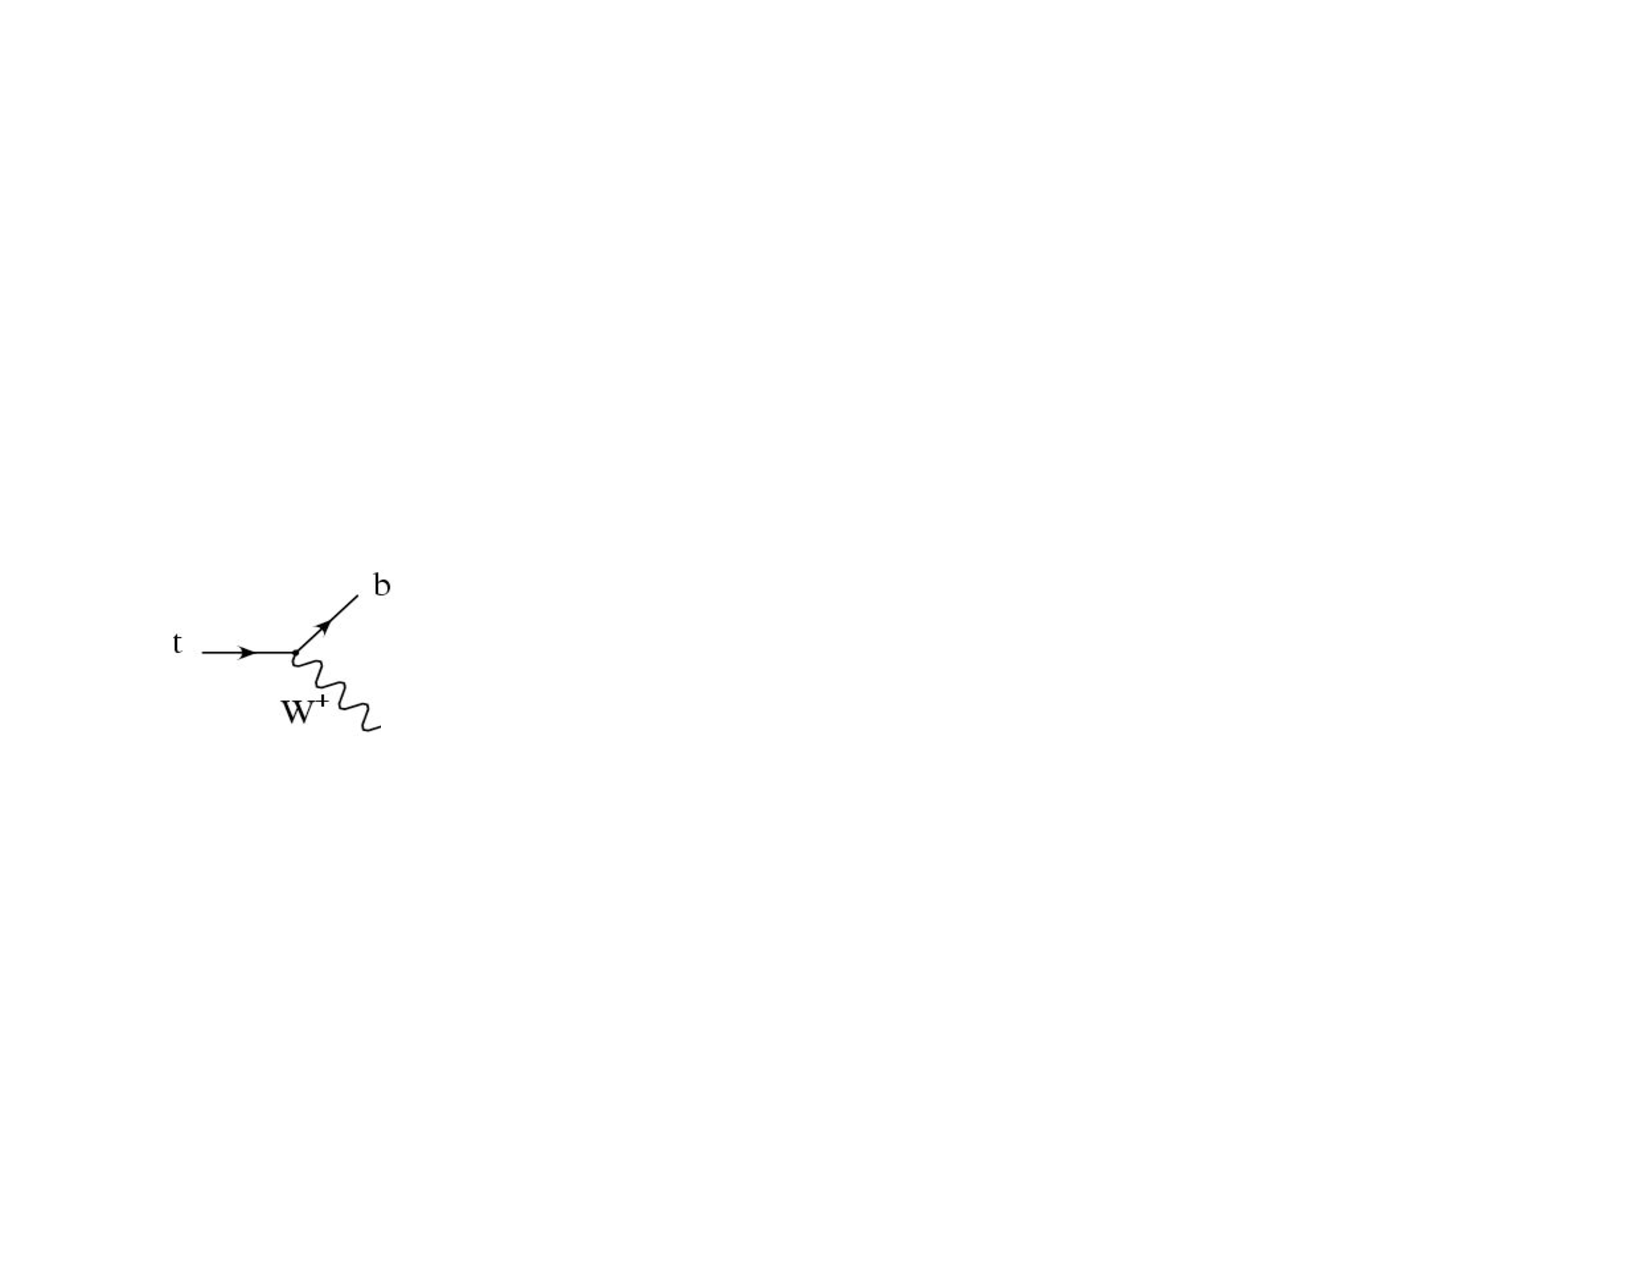
\includegraphics[width=0.5\textwidth]{topdecay.pdf}
\end{center}
\caption{An illustration of top decay via flavour changing neutral current.}
\label{fig:topdecay}
\end{figure}

\subsection{Quantum Chromodynamics (QCD)}

SU(3) is the symmetry group of the strong force. Particles which interact via
the strong force carry colour charge. Quarks come in 3 colours denoted r, g and 
b. There are 8 gluons which correspond to the 8 generators of SU(3). Gluons 
carry colour charge and so interact with each other. This is required by gauge 
invariance due to the non-abelian nature of SU(3). \\

\begin{figure}
\begin{center}
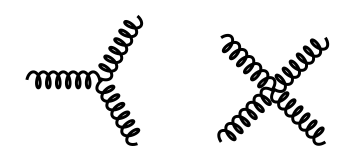
\includegraphics[width=0.8\textwidth]{gluons.png}
\end{center}
\caption{Gluon self-interactions occur because gluons carry colour charge. This
is required by gauge invariance due to the non-abelian nature of SU(3).}
\end{figure}

The Hadron Electron Ring Accelerator (HERA) made electron proton collisions to
determine the structure of the proton. Deep inelastic scattering in the ZEUS and
H1 detectors revealed that the structure functions of the proton are independent
of the momentum transfer, $Q^{2}$, and dependent only on $x = 
\frac{Q^{2}}{2p.q}$. This is called bjorken scaling and lead to the parton model 
in which the proton is made of partons which carry a fraction, $x$, of the 
proton momentum. Figure \ref{fig:dis} shows the independence of the 
cross-section with $Q^{2}$ over 5 orders of magnitude. \\

\begin{figure}
\begin{center}
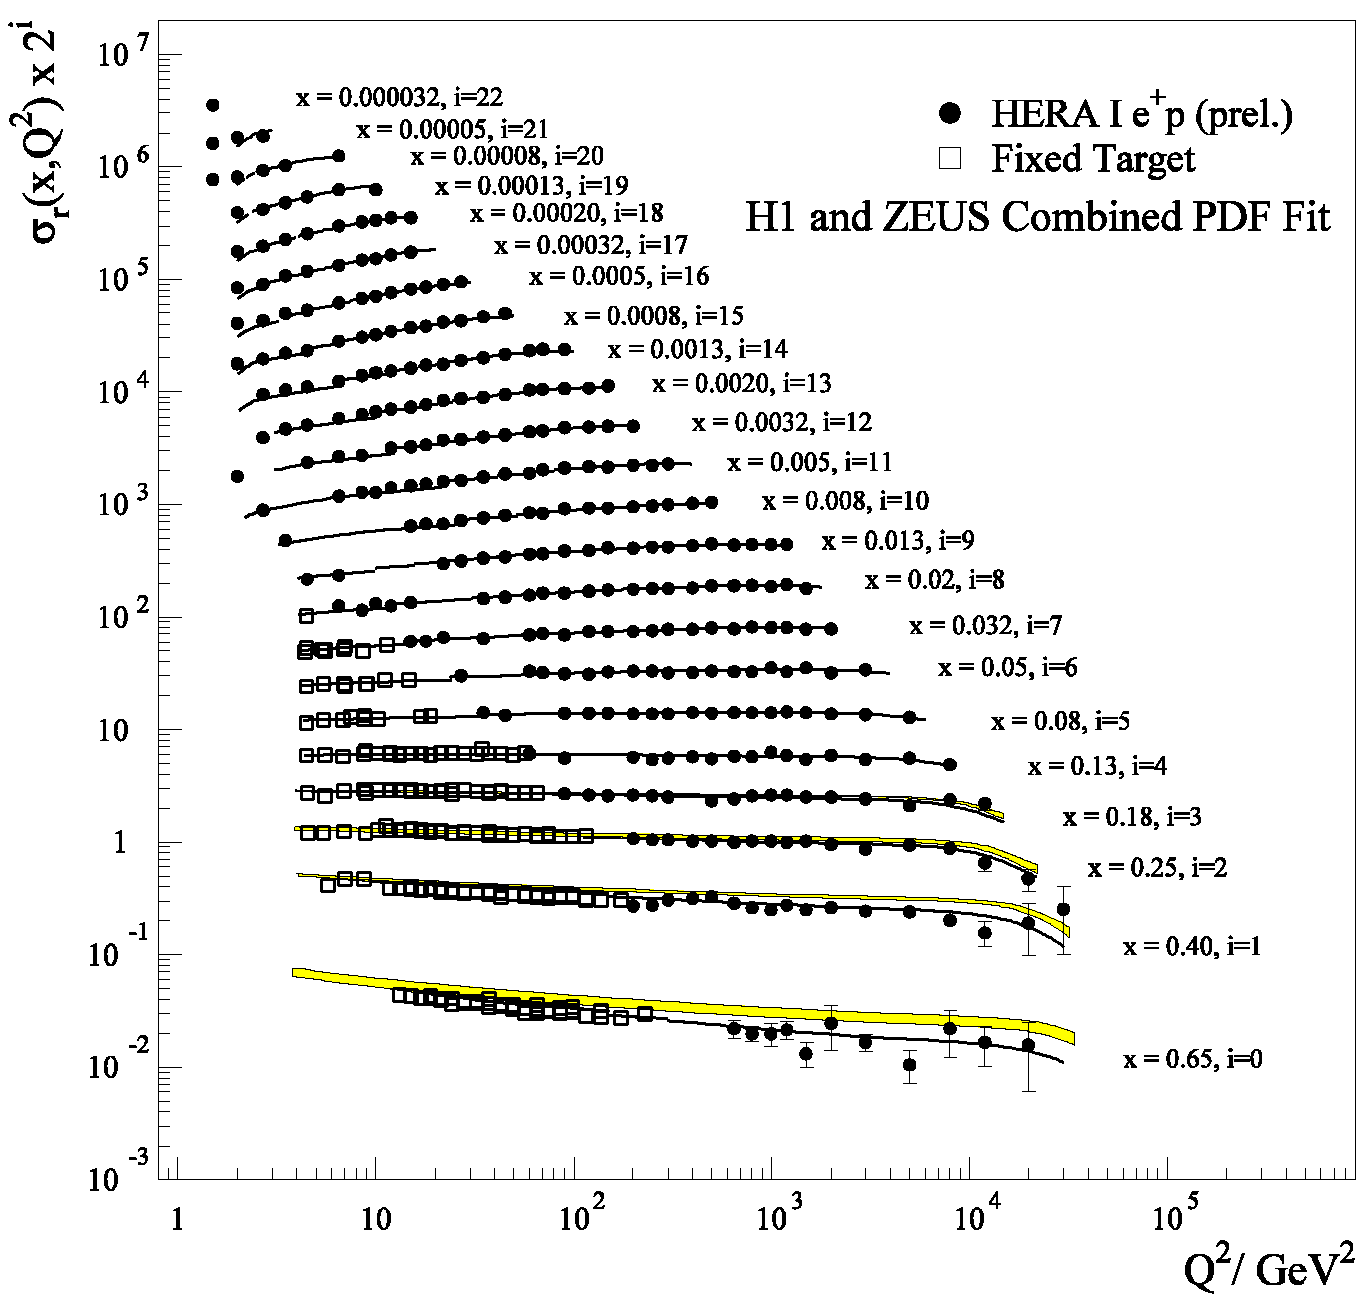
\includegraphics[width=\textwidth]{DIS-QCD.png}
\end{center}
\caption{The structure functions of the proton are independent of $Q^{2}$ over 5
orders of magnitude.}
\label{fig:dis}
\end{figure}

The Parton Density Functions (PDFs) are the probability distribution for the
fraction of the proton momentum carried by each parton. The PDFs need to be
known to make reliable Monte Carlo simulations and cross-section predictions for 
the LHC. Figure \ref{fig:pdfs} shows the parton density functions measured by H1 and
ZEUS. \\

\begin{figure}
\begin{center}
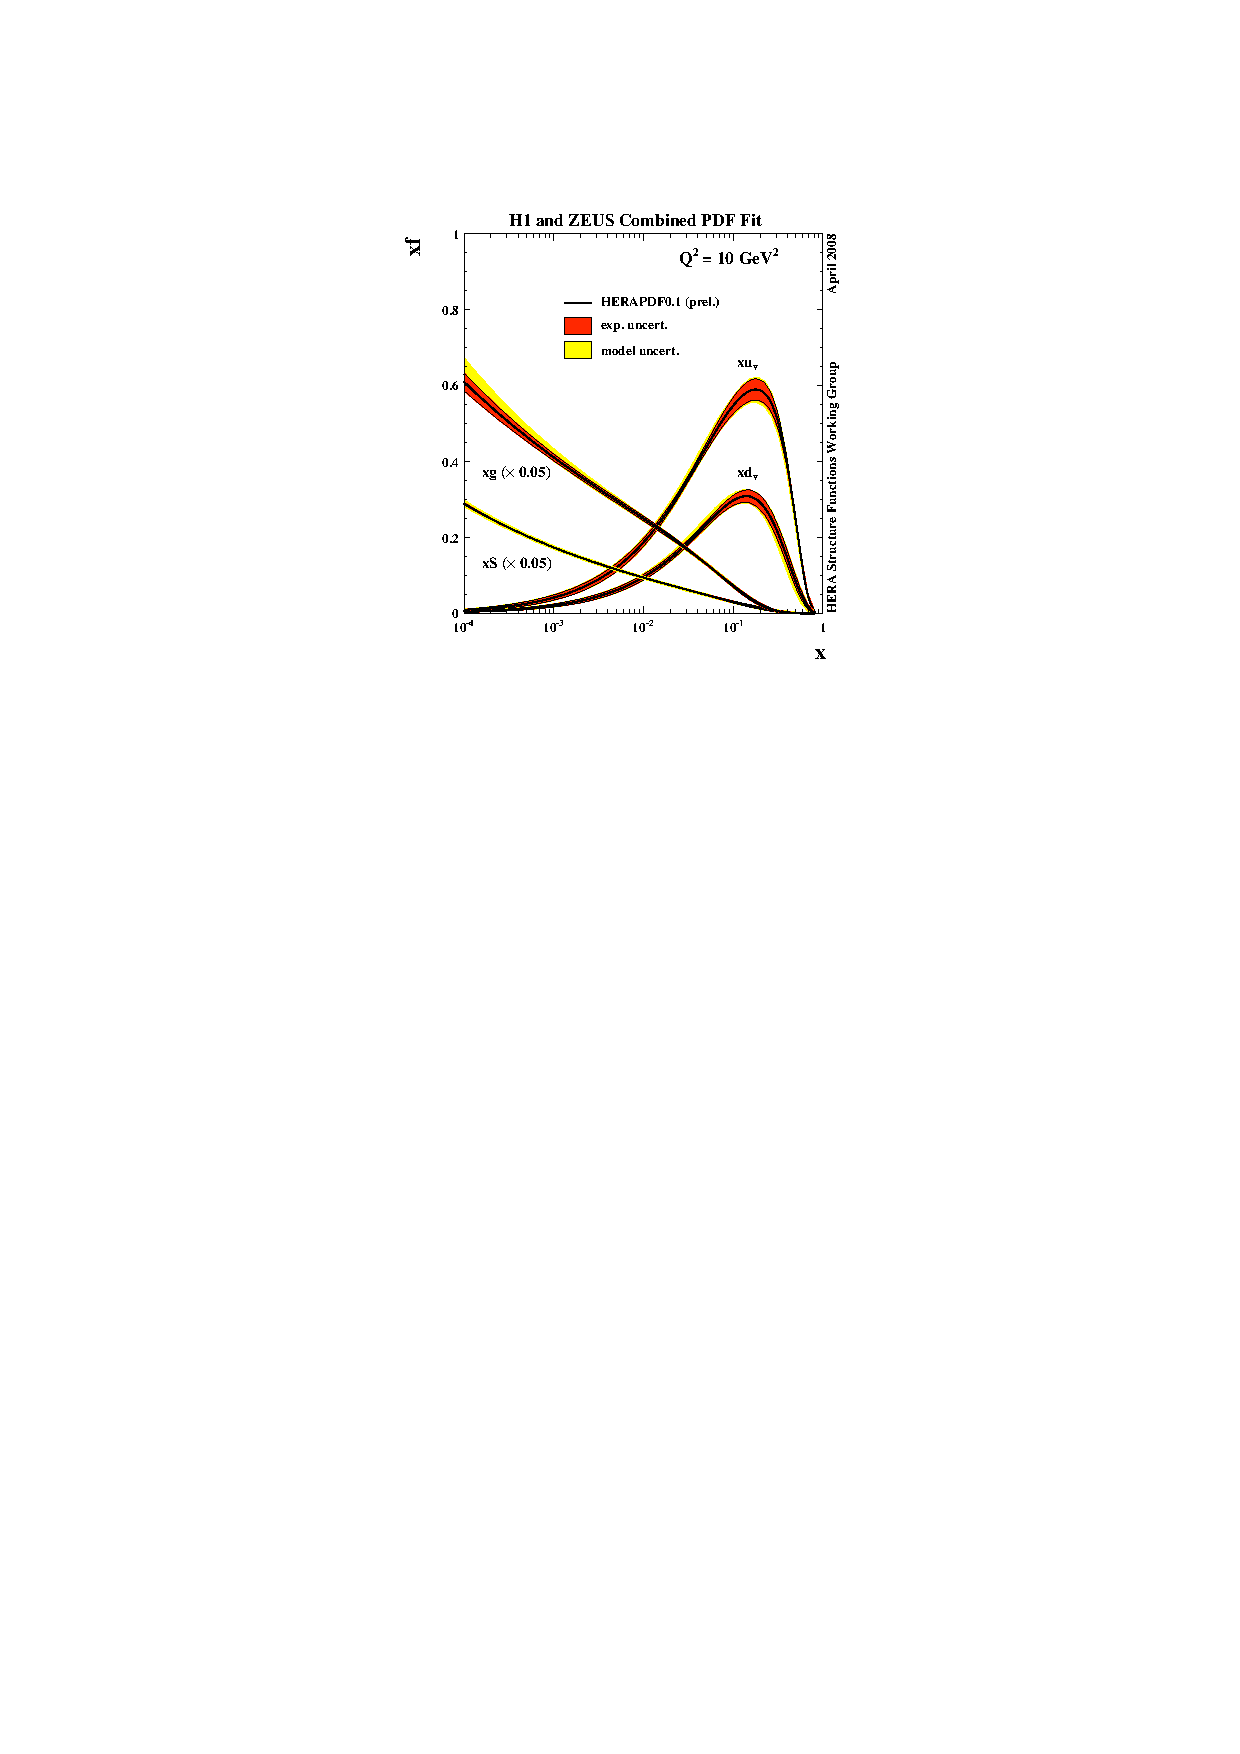
\includegraphics[width=0.8\textwidth]{PDFs.pdf}
\end{center}
\caption{The Parton Density Functions (PDFs) measured by H1 and ZEUS.}
\label{fig:pdfs}
\end{figure}

The coupling strength of the strong force varies with energy. The strong force 
is strong at low energies where quarks exist only in colourless bound states. 
This is known as confinement. At high energies the strong force becomes weaker 
as the partons behave as free particles. This is known as asymptotic freedom. 
Figure \ref{fig:coupling} shows the variation in coupling strength of the 
strong, weak and electromagnetic force as a function of energy.

\begin{figure}
\begin{center}
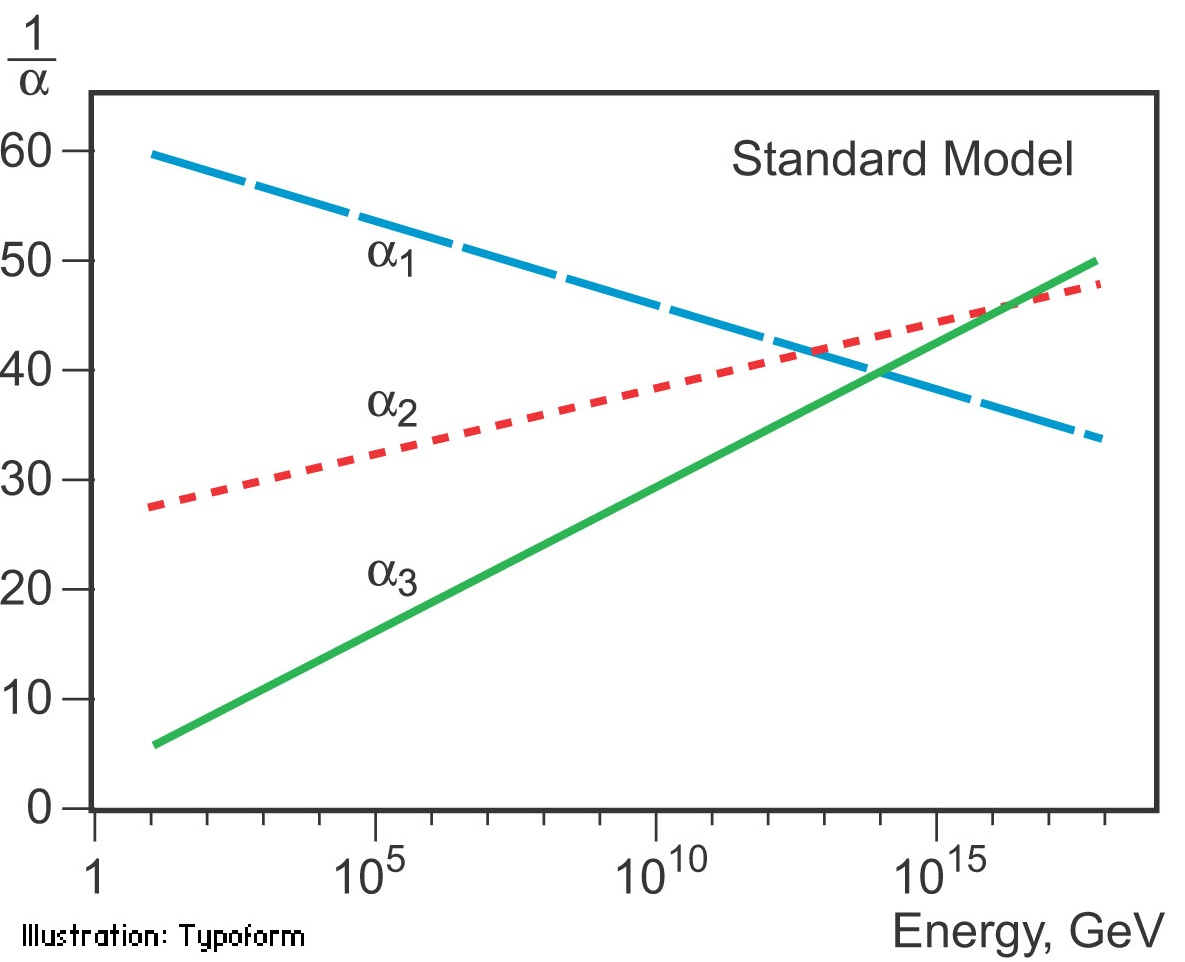
\includegraphics[width=0.8\textwidth]{coupling2.jpg}
\end{center}
\caption{The coupling strengths of the electromagnetic force, the weak force and
the strong force as a function of energy. Reproduced from \cite{nobel_2004}.}
\label{fig:coupling}
\end{figure}

\section{Motivation for new physics at the TeV scale}

The motivations for expecting the discovery of new physics at the TeV scale are
considered.

\subsection{WW scattering}

WW scattering (among other similar processes) has been observed at the Large 
Electron Positron (LEP) collider and the cross-section has been measured. 
Without additional couplings the interaction violates unitarity. The Higgs boson 
is one mechansim to mediate this interaction, but so far the Higgs has not been 
observed. Whatever the mechanism by which this interaction occurs it must be at 
the TeV energy scale to avoid violating unitarity.

\subsection{New energy scale}

This is simply the observation that we are exploring a higher energy scale than
has previously been explored so we can expect to find new things. In the same
way as when explorers explore a new land they can expect to see things they
have not seen before.

\subsection{Hierarchy Problem}

The hierarchy problem is fundamentally a problem of scale. There are two
fundamental energy scales in physics: the Electroweak scale ($\sim100\GeV$) and
the Planck scale ($\sim10^{18}\GeV$), where gravity becomes as strong as the 
gauge interactions. Certainly at the Planck scale the Standard Model will no
longer hold because a quantum treatment of gravity is needed. The Electroweak 
scale is well measured at colliders and the results form our current 
understanding of particle physics. It could be that there is no new physics 
between the two scales. Rejecting such a possibility means that the Higgs mass 
is alarmingly sensitive to any new physics. \\

\begin{figure}
\begin{center}
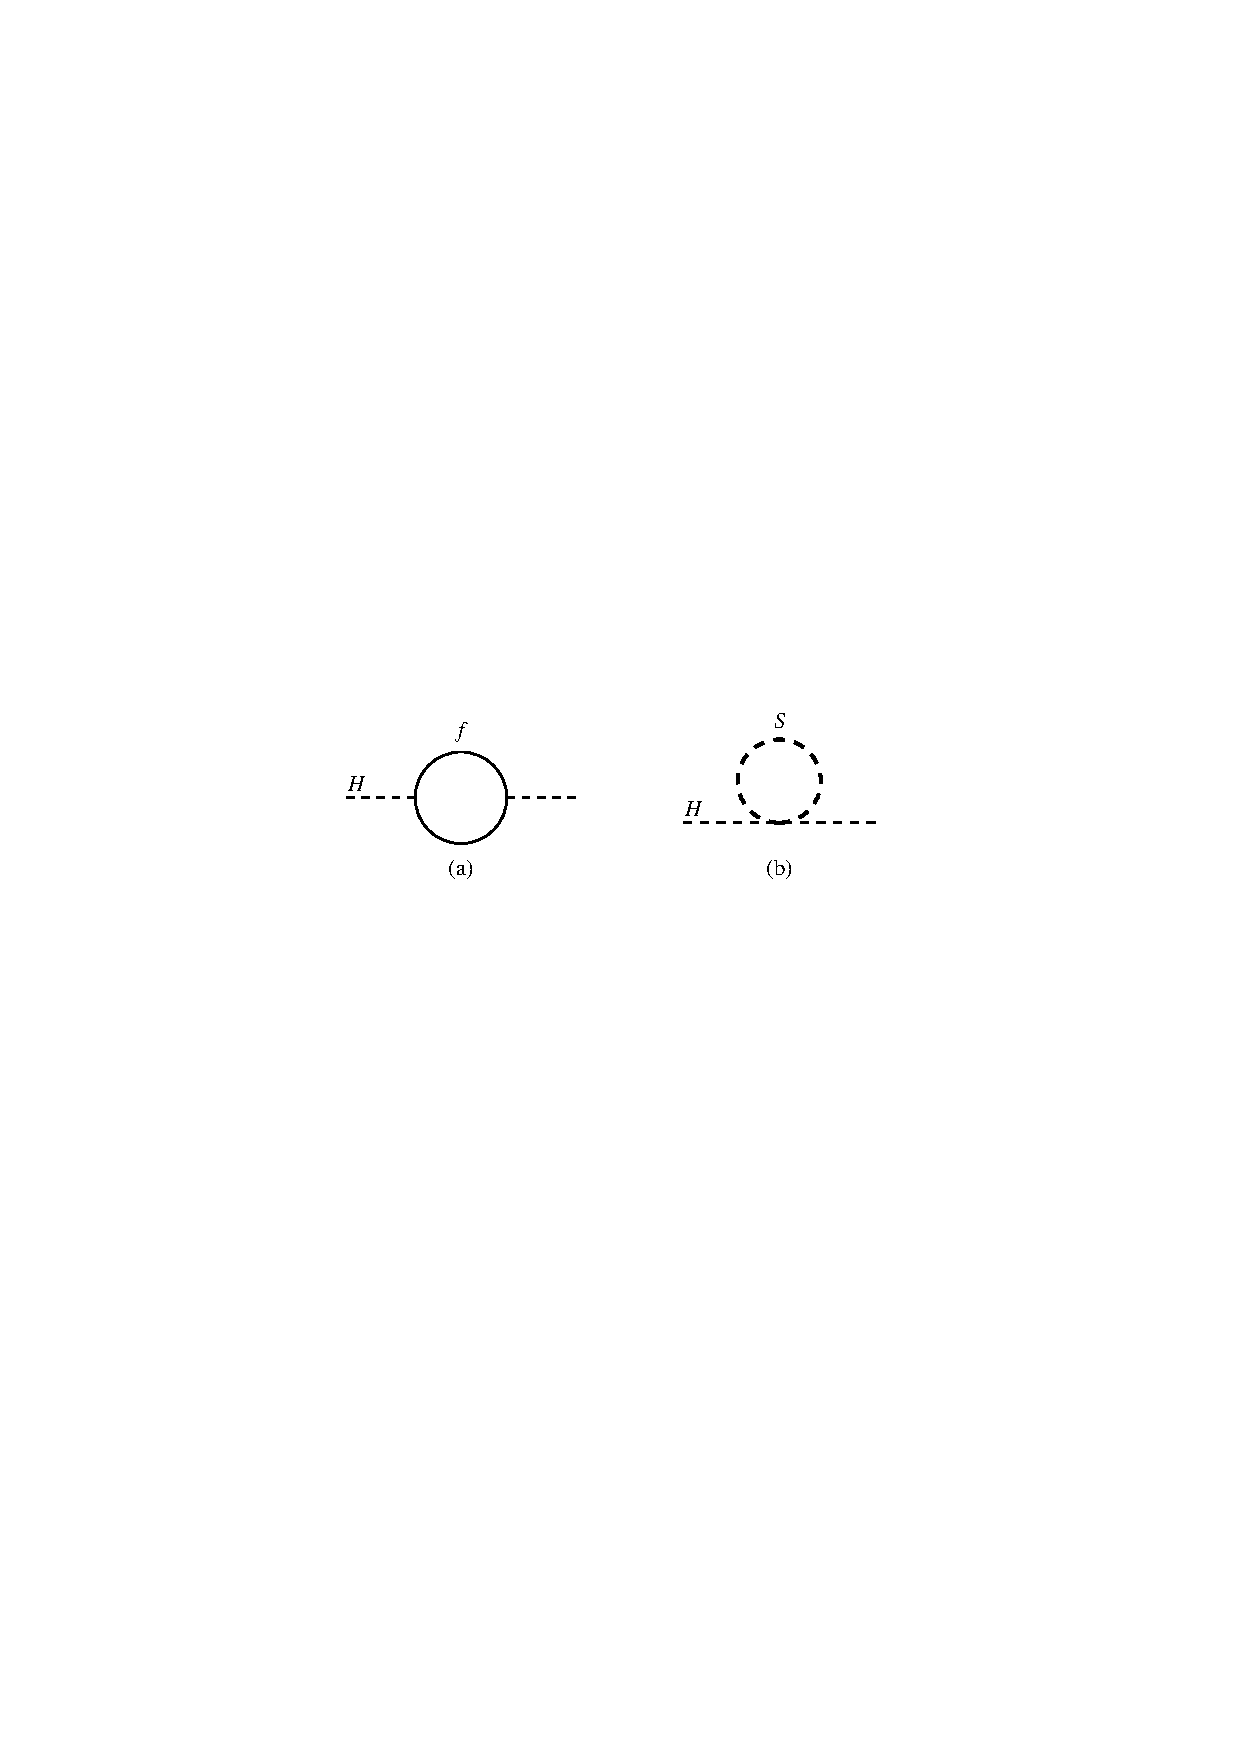
\includegraphics[width=0.8\textwidth]{higgs_loop.pdf}
\end{center}
\caption{Loop corrections to the Higgs mass squared $m_{H}^{2}$ from (a) a 
fermion f with mass $m_{f}$ and (b) a scalar S with mass $m_{S}$.}
\label{fig:higgs_loop}
\end{figure}

The one-loop quantum correction to the Higgs mass squared in Figure 
\ref{fig:higgs_loop}(a) with a fermion coupling $-\lambda_{f}\phi\bar{f}f$ and 
a cut-off energy $\Lambda$ is given by Equation \ref{eq:fermion_correction}.

\begin{equation}
\Delta m_{H}^{2} = -\frac{|\lambda_{f}|^{2}}{8\pi^{2}}\Lambda^{2} + ...
\label{eq:fermion_correction}
\end{equation}

For a scalar coupling $-\lambda_{S}|\phi|^{2}|S|^{2}$ and a cut-off $\Lambda$ 
the one-loop quantum correction to $m_{H}^{2}$ from Figure 
\ref{fig:higgs_loop}(b) is given by Equation \ref{eq:scalar_correction}.

\begin{equation}
\Delta m_{H}^{2} = \frac{\lambda_{S}}{16\pi^{2}}\Lambda^{2} + ...
\label{eq:scalar_correction}
\end{equation}

The one-loop quantum corrections to $m_{H}^{2}$ are quadratically divergent
depending on the cut-off used to do the calculation. In supersymmetry this
problem is solved by introducing a symmetry between fermions and bosons. For 
every Standard Model particle there is a supersymmetric partner which is a boson 
for fermions and a fermion for bosons. The fermions give a -1 contribution to 
$m_{H}^{2}$ while the bosons give a +1 contribution cancelling each other.

\subsection{Dark Matter candidates}

Only 5\% of the mass/energy in the universe is normal matter that we observe. 
The remainder is made up of dark matter (25\%) and Dark Energy (70\%). Dark
energy is an unknown that is introduced to explain the expansion of the
universe. Dark matter is well known. \\

The existence of dark matter is infered from its gravitational interaction with
normal matter. Dark matter was postulated as missing mass to account for the 
orbital velocities of galaxies in clusters. There have since been other 
observations that have confirmed the existence of dark matter including the 
rotational speed of galaxies and the bullet cluster. \\

The bullet cluster provides the best evidence yet on the nature of dark matter. 
It consists of two colliding clusters of galaxies. The visible matter (stars) 
pass straight through slowed only by gravitation. The hot gas which represents 
most of the normal matter is detected through X-rays. The hot gas slows more 
than the stars due to its electromagnetic interactions. Another piece of
information comes from gravitational lensing. In the absence of dark matter the
gravitational lensing is expected to follow the normal matter (i.e. the X-ray 
gas). However, the gravitational lensing is strongest in the separated regions
around the visible matter. This provides support to the idea that most of the 
mass of the galaxies is made up of collisionless dark matter. \\

If dark matter interacts through the weak force, then it could be observed at
the LHC. Dark matter may not interact weakly. Perhaps it interacts only 
gravitationally. Additionally it may not show up at the TeV scale. I will simply
make two statements which offer some support for the discovery of possible dark 
matter candidates at the LHC. Firstly, TeV scale weakly interacting masive 
particles give dark matter abundances in the universe at about the 
experimentally observed level. Secondly, SUSY (which is one of the popular 
theories of physics beyond the standard model) predicts a set of supersymmetric 
particles the lightest of which could be a dark matter candidate.

\section{Supersymmetry}

Supersymmetry (SUSY) proposes that for every particle there is a supersymmetric 
partner which is a boson for fermions and a fermion for bosons \cite{primer}. 
Such a symmetry ensures cancellation of the divergence in the Higgs boson mass. 
The operator Q which generates the supersymmetric transformations can be written 
as Equation \ref{eq:susy_operator}.

\begin{equation}
Q|\mbox{Boson}> = |\mbox{Fermion}> \hspace{10pt} Q|\mbox{Fermion}> = |\mbox{Boson}>
\label{eq:susy_operator}
\end{equation}

The forms of additional symmetries to the Poincare group are highly restricted
by the Coleman Mandula theorem \cite{coleman}. Supersymmetry is one of the few
possible symmetry extensions. \\ 

The Standard Model particles and their SUSY partners form supermultiplets as in
Equation \ref{eq:supermultiplets}. Since the particles within the
supermultiplets must maintain the gauge symmetries of the Standard Model, Q must 
commute with the internal symmetries of the Standard Model.

\begin{equation}
\left(\begin{array}{c}fermion\\sfermion\end{array}\right) \hspace{1cm}
\left(\begin{array}{c}gauge\hspace{3pt}boson\\gaugino\end{array}\right) \hspace{1cm}
\left(\begin{array}{c}graviton\\gravitino\end{array}\right)
\label{eq:supermultiplets}
\end{equation}

A straightforward implementation of supersymmetry would predict a whole new set
of particles with the same mass and same interactions as the Standard Model
particles. Since we do not observe these particles SUSY, if it exists, must be 
broken. The superpartners can then be at a higher mass scale. There are various
different schemes for SUSY breaking \cite{atchinson}. Here only Gauge Mediated 
SUSY Breaking (GMSB) is considered. \\

Another symmetry R-parity ($R_{P}$), defined in Equation \ref{eq:rparity}, is 
often introduced to SUSY models to preserve lepton number and baryon number. 
$R_{P}$ is +1 for Standard Model particles and -1 for supersymmetric partners.

\begin{equation}
R_{P} = (-1)^{3B+L+2S}
\label{eq:rparity}
\end{equation}

If R-parity is conserved, there are two important consequences:

\begin{itemize}
\item At colliders supersymmetric partners can only be produced in pairs.
\item The lightest supersymmetric particle (LSP) is stable.
\end{itemize}

The first point ensures that a supersymmetric particle always decays into 
another supersymmetric particle and that there are always two decay chains of 
supersymmetric particles in each supersymmetric event. The second point means 
that SUSY events contain missing energy since the LSP is not detected. The LSP 
also provides a possible dark matter candidate.

\section{Gauge Mediated SUSY breaking (GMSB)}

Under GMSB the messenger particles between the visible sector (Standard Model
and SUSY particles) and the hidden sector (responsible for the SUSY breaking)
are gauge particles. In the Minimal Supersymmetric Standard Model (MSSM) there 
are 6 parameters describing GMSB:

\begin{itemize}
\item $\Lambda$ -- the SUSY beaking scale. 
\item $M_{m}$ -- the mass scale of the messengers.
\item $N_{5}$ -- the number of messengers.
\item $\tan\beta$ -- the ratio of the higgs vacuum expectation values.
\item $\mbox{sign}(\mu)$ -- the sign of the higgsino mass term.
\item $C_{grav}$ -- the scale factor of the gravitino coupling.
\end{itemize}

SUSY events contain real Missing Transverse Energy ($\MET$) from the Lightest 
Supersymmetric Particle (LSP). In GMSB models with $N_{5} = 1$ and low
$\tan\beta$, the LSP is the gravitino ($\tilde{G}$) and the Next Lightest 
Supersymmetric Particle (NLSP) is the lightest neutralino 
($\tilde{\chi}_{1}^{0}$). The Neutralino decays into a photon and a gravitino 
$\tilde{\chi}_{1}^{0}\rightarrow\gamma\tilde{G}$. Since the two photons come from 
separate decay chains there is little correlation betweeen the two: they do not 
have a particular invariant mass nor a particular angular separation. \\

At lower $\sqrt{s}$, for example at LEP ($200\GeV$) and at the Tevatron
($500\GeV$), the GMSB cross section is lower and the dominant production 
mechanism is electroweak production through a W or a Z. The signature for 
electroweak production GMSB is $\gamma\gamma + \MET$. ALEPH \cite{aleph} at LEP 
($e^{+}e^{-}$ collider) and D0 \cite{d0} and CDF \cite{cdf} at the Tevatron 
($p\bar{p}$ collider) have published limits on electroweak production GMSB. \\

\begin{figure}
\begin{center}
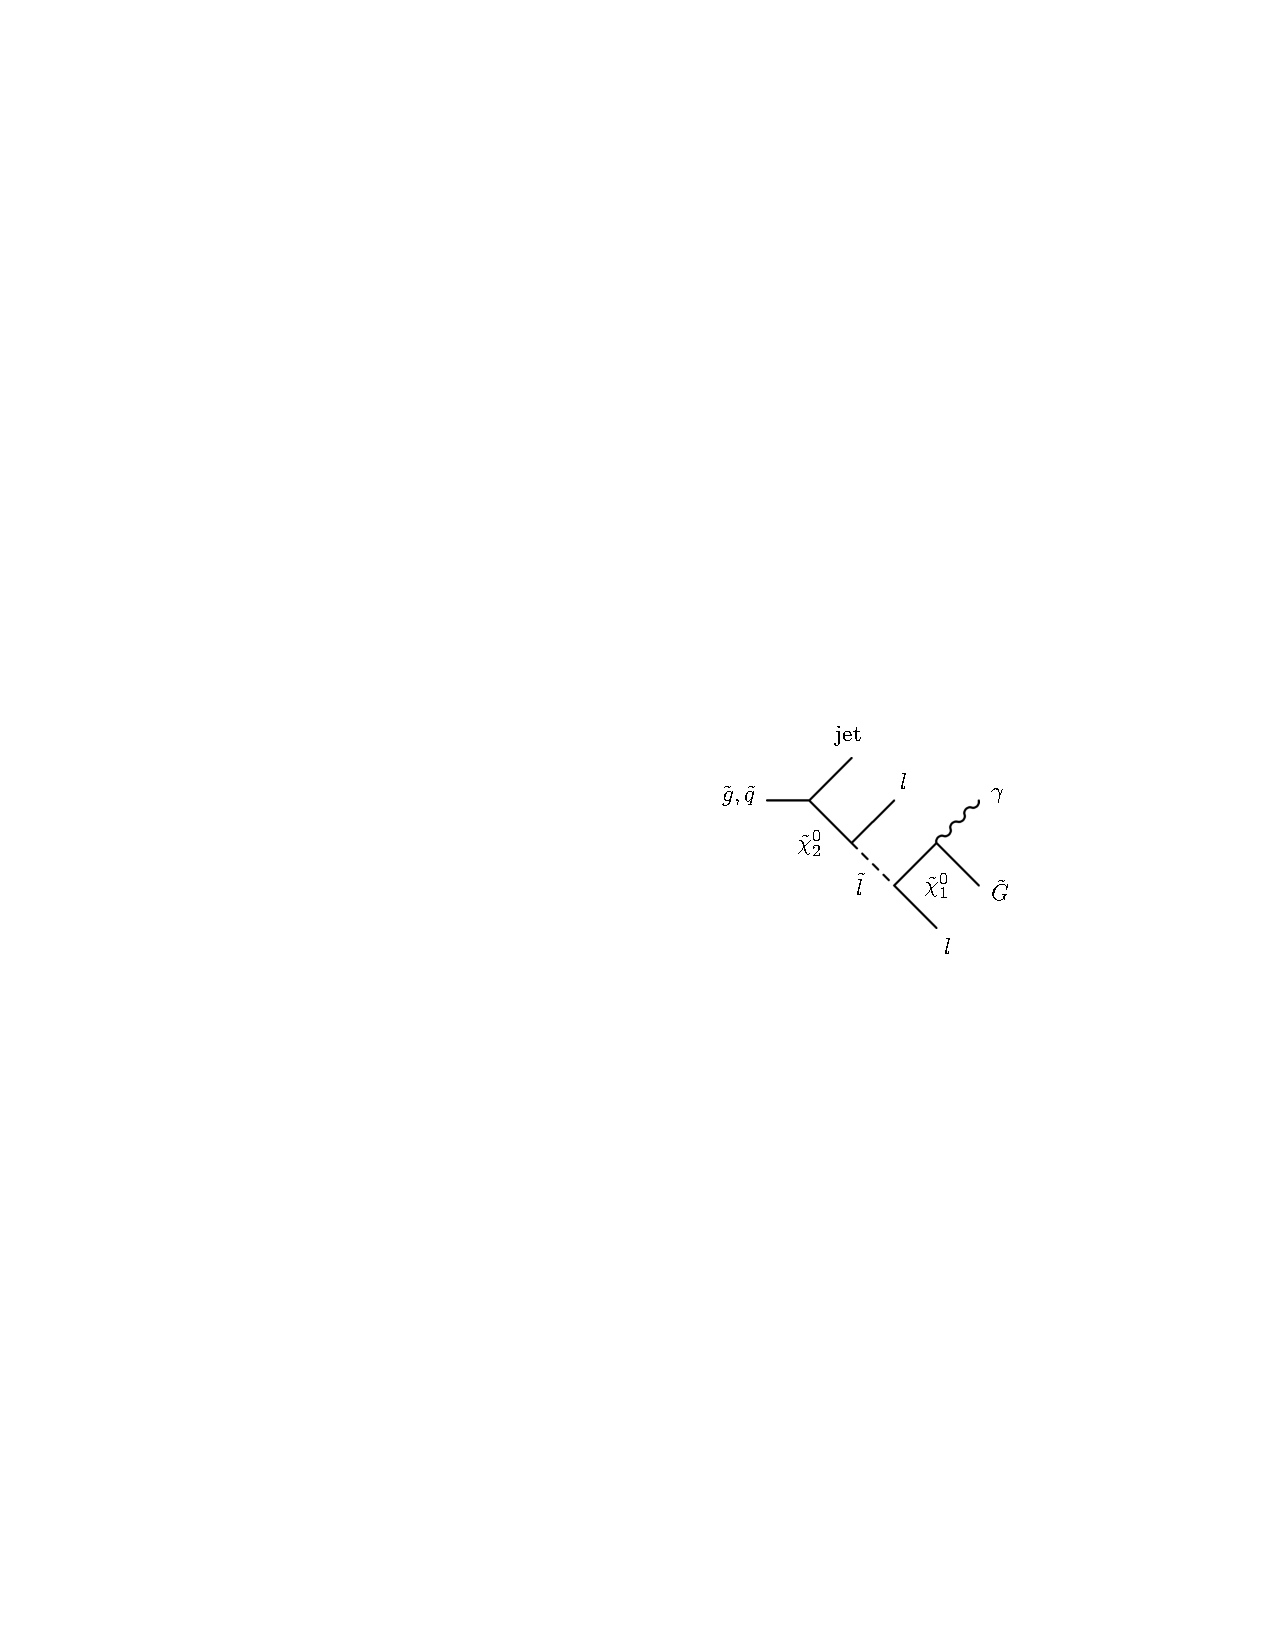
\includegraphics[width=\textwidth]{susy_decay_chain.pdf}
\end{center}
\caption{An example of a strong production SUSY decay chain. Reproduced from
\cite{gmsb_at_lhc}.}
\label{fig:susydecay}
\end{figure}

At the LHC energy ($7\TeV$) the cross section is higher and strong production is 
dominant. Figure \ref{fig:susydecay} shows an example of a strong production SUSY 
decay chain. Strong production events must contain at least two jets from the 
two squarks/gluions. Squarks decay to a quark and the next particle in the SUSY 
mass hierarchy ($\tilde{q}\rightarrow q\tilde{X}$) resulting in one jet. Gluinos 
decay to a quark anti-quark pair and the next particle in the SUSY mass 
hierarchy ($\tilde{g}\rightarrow q\bar{q}\tilde{X}$) resulting in two jets. The 
only previous limits on strong production GMSB come from ATLAS \cite{atlas} and 
CMS \cite{ra3} at the LHC. \\

